\documentclass[11pt]{article}
\usepackage[margin=1in]{geometry} 
\usepackage{amsmath,amsthm,amssymb,amsfonts}

\usepackage{mathpazo}
\usepackage{euler}
\usepackage{xcolor}
\usepackage{tikz}
\usetikzlibrary{matrix}
\usepackage{fancyhdr}
\pagestyle{fancy}

\newcommand{\N}{\mathbb{N}}
\newcommand{\Z}{\mathbb{Z}}
\newcommand{\Q}{\mathbb{Q}}
\newcommand{\R}{\mathbb{R}}
\newcommand{\C}{\mathbb{C}}
\newcommand{\M}[2]{\mathsf{M}_{#1}#2}
\newcommand{\im}{\operatorname{im}}
\newcommand{\eps}{\varepsilon}
\newcommand{\dpart}[2]{\frac{\partial#1}{\partial#2}}
\newcommand{\nat}[1]{[\![#1]\!]}
\newcommand{\natzero}[1]{\nat{#1}_0}
\newcommand{\adj}[1]{\operatorname{adj}(#1)}
\newcommand{\ip}[2]{\langle #1 , #2 \rangle}
\newcommand{\paint}[2]{\color{#1}{#2}}
\newcommand{\ol}{\overline}
\newcommand{\hook}[3]{\frac{\partial}{\partial x_{#1}}\Big\rvert_{#2}^{#3}}
\definecolor{red}{RGB}{244, 66, 66}

\renewcommand*{\proofname}{\paint{red}{Demostraci\'on}}
\newenvironment{theorem}[2][Teorema]{\begin{trivlist}
\item[\hskip \labelsep \paint{red}{{\bfseries #1}}\hskip \labelsep {\bfseries #2.}]}{\end{trivlist}}
\newenvironment{lemma}[2][Lema]{\begin{trivlist}
\item[\hskip \labelsep \paint{red}{{\bfseries #1}}\hskip \labelsep {\bfseries #2.}]}{\end{trivlist}}
\newenvironment{exercise}[2][Ejercicio]{\begin{trivlist}
\item[\hskip \labelsep \paint{red}{{\bfseries #1}}\hskip \labelsep {\bfseries #2.}]}{\end{trivlist}}
\newenvironment{obs}[2][Observaci\'on]{\begin{trivlist}
\item[\hskip \labelsep \paint{red}{{\bfseries #1}}\hskip \labelsep {\bfseries #2.}]}{\end{trivlist}}
\newenvironment{reflection}[2][Resoluci\']{\begin{trivlist}
\item[\hskip \labelsep {\bfseries #1}\hskip \labelsep {\bfseries #2.}]}{\end{trivlist}}
\newenvironment{proposition}[2][Proposici\'on]{\begin{trivlist}
\item[\hskip \labelsep {\bfseries #1}\hskip \labelsep {\bfseries #2.}]}{\end{trivlist}}
\newenvironment{corollary}[2][Corolario]{\begin{trivlist}
\item[\hskip \labelsep {\bfseries #1}\hskip \labelsep {\bfseries #2.}]}{\end{trivlist}}

%-----------------------

\title{
\LARGE{\paint{red}{Geometr\'ia Diferencial}}
\\
\vspace{0.5pt}
\small{\paint{red}{Ejercicios para Entregar - Pr\'actica 2}}
}
\author{\paint{red}{Guido Arnone}}
\date{}
\lhead{Guido Arnone}
\rhead{Pr\'actica 2}

\begin{document}

\maketitle

\begin{center}
\paint{red}{\large{Sobre los Ejercicios}}
\end{center}
Adem\'as del ejercicio $\paint{red}{(9)}$, elej\'i resolver los ejercicios $\paint{red}{()}$ y $\paint{red}{(12)}$. Con la intenci\'on de hacer m\'as legibles a las resoluciones, algunos argumentos est\'an escritos en forma de lemas que preceden a cada ejercicio.
\begin{center}
$\paint{red}{
\rule{400pt}{0.5pt}
}$
\vspace{35pt}
\end{center}

\begin{exercise}{9} Sea $M$ una variedad diferenciable de dimensi\'on $n$ y $\mathcal{A}$ su atlas maximal. Sea $TM=\bigcup_{p\in M}M_{p}$ y sea $\pi :TM\to M$ la funci\'on tal
que $\pi (v)=p$ si $v\in M_{p}$. Para cada $(U,x)\in \mathcal{A}$, sea
$TU=\bigcup_{p\in U}M_{p}\subset TM$ y $\ol{x}:TU\to
x(U)\times \R^{n}$ la funci\'on tal que
  \[
  \ol{x}(v)=(x(\pi (v)),v(x^{1}),\dots ,v(x^{n}))
  \]
cada vez que $v\in TU$.
\begin{itemize}
\item[(a)] La funci\'on $\ol{x}:TU\to x(U)\times \R^{n}$ es una biyecci\'on
con inversa tal que
  \[
  \ol{x}^{-1}(a,b^{1},\dots,b^{n})
        = \sum_{i=1}^{n}b^{i}\frac{\partial}{\partial x^{i}}\Big|_{x^{-1}(a)}
  \]
para cada $a\in x(U).$

\item[(b)] Si $(U,x)$,~$(V,y)\in \mathcal{A}$ y $U\cap V\neq\emptyset$, entonces $\ol{x}(TU\cap
TV) = x(U\cap V)\times\R^{n}$ es un abierto de $\R^{2n}$ y 
la biyecci\'on $\ol{x}\circ \ol{y }^{-1}:y(U\cap V)\times\R^{n}\to x(U\cap V)\times 
\R^{n}$ es un difeomorfismo.

\item[(c)] El conjunto $TM$ admite una estructura diferenciable que lo transforma en
una variedad diferenciable de dimensi\'on $2n$, con atlas
  \[
  \ol{\mathcal{A}}=\{(TU,\ol{x}):(U,x)\in\mathcal{A}\}.
  \]

\item[(d)] Con respecto a esta estructura diferenciable, la proyecci\'on $\pi :TM\to M$ es diferenciable.
\end{itemize}
\end{exercise}
\begin{proof} Hacemos cada inciso por separado,
\begin{itemize}
\item[(a)] Sean $(a,b) = (a, b^1, \dots, b^n) \in x(U) \times \R^n$ y $h(a,b) := \sum_{i=1}^nb^i \frac{\partial}{\partial x_i}|_{x^{-1}(a)}$. Como esta \'ultima expresi\'on es una combinaci\'on lineal de derivaciones en $x^{-1}(a)$, luego $h(a,b)$ es una derivaci\'on en $x^{-1}(a)$. Por lo tanto, $h(a,b) \in M_{x^{-1}(a)}$ y as\'i $x\pi(h(a,b)) = xx^{-1}(a) = a$. Adem\'as, si $\pi_j : \R^n \to \R$ es la proyecci\'on en la $j$-\'esima coordenada, luego para cada $j \in \nat{n}$ es $x^j = \pi_jx$ y entonces
\begin{align*}
h(a,b)(x^j) &= \left(\sum_{i=1}^nb^i \hook{i}{x^{-1}(a)}{} \right)(x^j) = \sum_{i=1}^nb^i \hook{i}{x^{-1}(a)}{}(x^j) = \sum_{i=1}^nb^i \frac{\partial (x^jx^{-1})}{\partial x_i}\Big|_a \\
& = \sum_{i=1}^nb^i \frac{\partial \pi_j}{\partial x_i}\Big|_a =  \sum_{i=1}^nb^i \delta_{ij} = b^j.
\end{align*}
Concluimos as\'i que $\ol{x}(h(a,b)) = (a,b) \in x(U) \times \R^n$. Rec\'iprocamente si $v \in M_p$ con $p \in U$, luego
\begin{align*}
h(\ol{x}(v)) & = h(x\pi(v),v(x^1),\dots,v(x^n)) = \sum_{i=1}^nv(x^i)\hook{i}{x^{-1}(x\pi(v))}{} = \\
& = \sum_{i=1}^nv(x^i)\hook{i}{p}{}.
\end{align*}
Esto \'ultimo coincide justamente la expresi\'on de $v$ en la base $\big\{\hook{i}{p}{}\big\}_{i=1}^n$, lo que termina de probar que en efecto $h = \ol{x}^{\ -1}$.
\item[(b)] Notemos en primer lugar que como $U \cap V$ es abierto y $x$ homeomorfismo, luego $x(U\cap V)$ es abierto, y as\'i $x(U \cap V) \times \R^n$ es abierto en $\R^{2n}$. Por definici\'on, es $TU \cap TV = T(U \cap V)$ y $\ol{x|_{U \cap V}} = \ol{x}|_{T(U \cap V)}$ as\'i que como $\ol{x|_{U \cap V}}$ es sobreyectiva (pues $x|_{U \cap V}$ es otra carta de $M$), por $\paint{red}{(b)}$ en efecto es $\ol{x}(TU \cap TV) = x(U \cap V) \times \R^n$. Veamos ahora que $\ol{x}\ol{y}^{-1}$ es un difeomorfismo. Como $\ol{x}$ e $\ol{y}$ son biyectivas, basta ver que las composiciones $\ol{x}\ol{y}^{-1}$ y $\ol{y}\ol{x}^{-1}$ son diferenciables. Por simetr\'ia (ya que podemos intercambiar los roles de $x$ e $y$) basta probar una, lo hacemos para $\ol{x}\ol{y}^{-1}$. Por un c\'alculo directo, si $(a,b) \in y(U\cap V) \times \R^n$ y $\pi_j : \R^n \to \R$ una vez m\'as es la proyecci\'on en la $j$-\'esima coordenada, luego para cada $j \in \nat{n}$ es $x^jy^{-1} = \pi_jxy^{-1} = (xy^{-1})^j$, y entonces
\begin{align*}
\ol{y}^{-1}(a,b)(x^j) &= \sum_{i=1}^n b^i \frac{\partial}{\partial y_i}\Big|_{y^{-1}(a)}(x^j) = \sum_{i=1}^nb^i \frac{\partial x^jy^{-1}}{\partial x_i}\Big|_a \\ & = \sum_{i=1}^nb^i \frac{\partial (xy^{-1})^j}{\partial x_i}\Big|_a = [\mathbb{J}(xy^{-1})_a \cdot b]_j.
\end{align*}
con $\mathbb{J}(xy^{-1})_a$ la matriz jacobiana de $xy^{-1}:y(U \cap V) \subset \R^n \to x(U \cap V) \subset \R^n$ en el punto $a \in y(U \cap V)$. Por lo tanto, usando que por $\paint{red}{(a)}$ es $\pi \ol{y}^{-1}(a,b) = y^{-1}(a)$, luego
\begin{align*}
x\ol{y}^{-1}(a,b) & = (x\pi(\ol{y}^{-1}(a,b)),\ol{y}^{-1}(a,b)(x^1), \dots, \ol{y}^{-1}(a,b)(x^n)) \\ 
& = (xy^{-1}(a),[\mathbb{J}(xy^{-1})_a \cdot b]_1, \dots, [\mathbb{J}(xy^{-1})_a \cdot b]_n)\\
& = (xy^{-1}(a),\mathbb{J}(xy^{-1})_a \cdot b).
\end{align*}
Como $M$ es variedad diferenciable, luego $xy^{-1}$ es suave y entonces $a \mapsto \mathbb{J}(xy^{-1})_a$ es suave. De \'esto \'ultimo tenemos que $(a,b) \mapsto \mathbb{J}(xy^{-1})_a \cdot b$ es suave\footnote{Esto es porque en cada componente $(a,b) \mapsto \mathbb{J}(xy^{-1})_a \cdot b$ coincide con $(a,b) \mapsto \sum_{i=1}^nb^i \frac{\partial (xy^{-1})^j}{\partial x_i}\Big|_a$ que es una suma de productos de proyectar a $\mathbb{J}(xy^{-1})$ o $(a,b) \mapsto b$ en alguna coordenada, y todas las funciones involucradas son suaves.}, por lo que concluimos que $\ol{x}\ol{y}^{-1}$ es diferenciable.
\item[(c)] En primer lugar, veamos que la colecci\'on $\mathcal{T} = \{TU : U \subset M \text{ abierto}\}$ es una topolog\'ia que hace de $TM$ una variedad topol\'ogica. Antes que nada, observemos que si $(U_i)_{i \in I}$ es una familia de abiertos de $M$, luego por definici\'on es $T(\bigcup_{i \in I}U_i) = \bigcup_{i \in I}TU_i$ y $T(\bigcap_{i \in I}U_i) = \bigcap_{i \in I}TU_i$. En particular, $M$ y $\emptyset$ son abiertos asi que $\emptyset = T\emptyset,TM \in \mathcal{T}$ y los conjuntos $TU$ son cerrados por interesecciones finitas y uniones arbitrarias, ya que los abiertos de $M$ lo son. As\'i, $\mathcal{T}$ es una topolog\'ia para $M$. A continuaci\'on, veamos que $TM$ resulta Hausdorff y posee una base contable. 
\item[(d)] Sea $v \in TM$ con $p \in M$ tal que $v \in M_p$. Ahora, tomemos una carta $(U,x)$ de $M$ con $\pi(v) = p \in U$. Por $\paint{red}{(c)}$ sabemos que $(TU, \ol{x})$ es una carta de $v$, y por definici\'on de $TU$ es tambi\'en $\pi(TU) = U$. Por lo tanto, resta ver que \textit{bajando} con estas cartas la funci\'on que resulta es diferenciable entre abiertos eucl\'ideos. Es decir, basta con probar que la flecha punteada del siguiente diagrama conmutativo es diferenciable:
\begin{center}
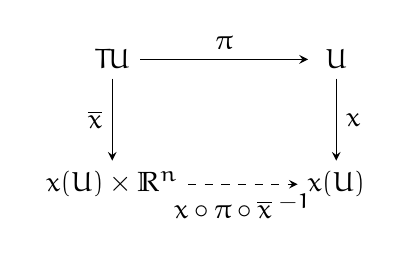
\begin{tikzpicture}
  \matrix (m) [matrix of math nodes,row sep=3em,column sep=4em,minimum width=2em]
  {
     TU & U\\
     x(U) \times \R^n & x(U)\\};
  \path[-stealth]
    (m-1-1) edge node [above] {$\pi$} (m-1-2)
            edge node [left] {$\ol{x}$}  (m-2-1)
    (m-2-1) edge [dashed] node [below] {$x\circ \pi \circ \ol{x}^{\ -1}$} (m-2-2)
    (m-1-2) edge node [right] {$x$} (m-2-2);
\end{tikzpicture}
\end{center}
Notemos que para todo $v \in TU$, el vector $x \circ \pi(v)$ coincide exactamente con las primeras $n$ coordenadas de $\ol{x}(v)$ por definici\'on de \'esta \'ultima. Notando $\pi_1 : (p,q) \in \R^n \times \R^n \mapsto p \in \R^n$ es entonces $x\circ \pi \circ \ol{x}^{\ -1} = \pi_1|_{x(U) \times \R^n} \circ \ol{x} \circ \ol{x}^{\ -1}  = \pi_1|_{x(U) \times \R^n}$, y esta \'ultima es diferenciable ya que es la restricci\'on al abierto $x(U) \times \R^n$ de la funci\'on diferenciable $\pi_1$.
\end{itemize}
\end{proof}

\begin{obs}{1} Sea $M$ una variedad diferenciable, $f \in C^\infty(M)$ una funci\'on constante y $v : C^\infty(M) \to \R$ una derivaci\'on en $p \in M$. Entonces, $v(f) = 0$. En efecto, si notamos $1 : M \to \R$ a la funci\'on constantemente $1$, luego
\begin{align*}
v(1) = v(1 \cdot 1) \stackrel{(Leibniz)}{=} 1(p)v(1) + 1(p)v(1) = 2v(1).
\end{align*}
Esto implica $v(1) = 0$. Si ahora $f$ vale constantemente $\mu \in \R$, entonces 
\begin{align*}
v(f) = v(\mu \cdot 1) = \mu v(1) = 0
\end{align*}
como afirmamos.
\end{obs}

\begin{lemma}{2} Sea $f : X \to Y$ una funci\'on con $X$ un espacio topol\'ogico conexo. Si $f$ es localmente constante, entonces es constante.
\end{lemma}
\begin{proof} Notemos que si $y \in \im f$, el conjunto $E_y := f^{-1}(y) = \{x \in X : f(x) = y\}$ es abierto: si $z \in E_y$, por hip\'otesis existe un abierto $U \ni z$ donde $f$ es constante, y como $f(z) = y$ luego $f$ es constantemente $y$ en todo $U$. Por lo tanto, es $z \in U \subset E_y$. Es claro adem\'as que estos conjuntos son disjuntos, pues si $z \in E_y \cap E_{y'}$ luego $y = f(z) = y'$. Por \'ultimo, como 
\begin{align*}
X = \bigsqcup_{y \in \im f}E_y
\end{align*}
es una escritura de $X$ como uni\'on de abiertos disjuntos no vac\'ios y $X$ es conexo, necesariamente es $\#\im f = 1$. Esto dice que $f$ es una funci\'on constante. 
\end{proof}

\begin{exercise}{12} Sean $M$ y $N$ variedades diferenciables y sea $f:M\to N$ una funci\'on
diferenciable.
\begin{itemize}
\item Si $f$ es constante, entonces $f_{\ast p}=0$ para todo $p\in M$.

\item Si $M$ es conexa y $f_{\ast p}=0$ para todo $p\in M,$ entonces $f$ es
constante.
\end{itemize}
\end{exercise}

\begin{proof} Notaremos $c_q : M \to N$ a la funci\'on que vale constantemente $q$. Definimos tambi\'en $m := \dim M$ y $n := \dim N$. Supongamos en primer lugar que $f = c_q$. Sea $p \in M$ y veamos que $f_{\ast p}$ es nula. Dada una derivaci\'on $v : C^\infty(M) \to \R$ en $p$ y $g \in C^\infty(M)$, luego es
\begin{align*}
f_{\ast p}(v)(g) =  v(- \circ f)(g) = v(gf) = v(gc_q) = v(c_{g(q)}) = 0,
\end{align*}
con esta \'ultima igualdad dada por la $\paint{red}{\text{Observaci\'on $1$}}$. Como la derivaci\'on $f_{\ast p}(v)$ se anula en toda funci\'on, tenemos que $f_{\ast p}(v) = 0$. Como $f_{\ast p}$ se anula en toda derivaci\'on, luego $f_{\ast p} = 0$ y esto vale para cualquier punto $p \in M$. Supongamos ahora que $M$ es conexa y veamos para este caso la afirmaci\'on rec\'iproca. Sea entonces $p \in M$ y veamos que existe un entorno abierto de $p$ donde $f$ es constante. Consideramos ahora una carta $(V,\psi)$ de $N$ con $f(p) \in V$ y una carta $(U,\varphi)$ de $M$ con $p \in U \subset f^{-1}(V)$ y $U$ conexo\footnote{Como $f$ es continua luego $f^{-1}(V)$ es abierto y entonces $f^{-1}(V) \cap U$ es un abierto de $M$ que contiene a $p$. Luego $f^{-1}(V) \cap U$ es un abierto en $U$, y como \'este es homeomorfo a un abierto eucl\'ideo, luego $f^{-1}(V) \cap U$ lo es tambi\'en. En particular tenemos un entorno conexo $\tilde{U}$ de $p$ contenido en $f^{-1}(V) \cap U$. Luego la restricci\'on de la carta a $\tilde{U}$ es una carta que cumple lo que pedimos. Por lo tanto, podemos sin p\'erdida de generalidad asumir directamente a $U$ conexo con $U \subset f^{-1}(V)$.}. Luego, los \textit{ganchos} $\bigg\{\hook{i}{q}{\varphi}\bigg\}_{i=1}^n$ son una base de $T_qM$ para cada $q \in U$. Por hip\'otesis, si $g \in C^\infty(N)$ y $v$ es una derivaci\'on en $q$, luego $v(gf) = f_{\ast q}(v)(g) = 0$. En particular, tenemos entonces que
\begin{align*}
\hook{i}{q}{\varphi}(gf) = \frac{\partial gf\varphi^{-1}}{\partial x_i}\bigg\rvert_{\varphi^{-1}(q)} = 0
\end{align*}
para todo $i \in \nat{m}$ y $q \in U$. Es decir, la funci\'on diferenciable $gf\varphi^{-1} : \varphi^{-1}(U) \to \R$ tiene gradiente nulo. Como $U$ es conexo y $\varphi$ es homeomorfismo, luego $\varphi^{-1}(U)$ es conexo. Como $gf\varphi^{-1}$ tiene gradiente nulo y dominio conexo luego es constante:
\begin{align*}
gf\varphi^{-1}(x) = \mu_{g} \in \R \quad (\forall x \in \varphi^{-1}(U)).
\end{align*}
Equivalentemente, es $gf \equiv c_{\varphi(\mu_g)}$ en $U$ para cada $g \in C^\infty(N)$. Ahora, para cada $i \in \nat{n}$ consideramos $\ol{\psi}^i \in C^\infty(N)$ tal que $\ol{\psi}^i|_V = \psi^i$. As\'i, existen constantes $c_1, \dots, c_n \in \R$ tales que $\ol{\psi}^if \equiv c_i$ en $U$ y como $f(U) \subset V$ es entonces
\begin{align*}
c_i \equiv \ol{\psi}^i|_V \circ f\Big|_U^V = \psi^i \circ f\Big|_U^V
\end{align*}
en $U$ para cada $i \in \nat{n}$. Por lo tanto, es $\psi f \big|_U^V \equiv c$. Como $\psi$ es homeomorfismo, luego $f \big|_U^V \equiv \psi(c)$. As\'i, vemos que $f$ es constante en el abierto $U \ni p$. Como $p$ era arbitrario, concluimos que $f$ es localmente constante y como $M$ es conexa, el $\paint{red}{\text{Lema $2$}}$ nos dice que $f$ resulta constante.
\end{proof}

\end{document}
